\section{Цель работы}
\begin{enumerate}
	\item Изучение вынужденных колебаний и явления резонанса напряжений в последовательном колебательном контуре.
	\item Построение резонансной кривой и определение резонансной частоты.
	\item Определение активного сопротивления и добротности колебательного контура.
\end{enumerate}

\section{Объект исследования}
Объект исследования - вынужденные электромагнитные колебания,
возникающие в последовательном колебательном контуре.
\section{Метод экспериментального исследования}
Многократное прямое измерение колебаний в колебательном контуре.

\section{Рабочие формулы и исходные данные}
\begin{enumerate}
	\item Добротность контура \(Q = \frac{\Omega_0}{\Delta \Omega}\),
	      где \(\Omega_0\) -- резонансная частота, \(\Delta \Omega\) -- ширина резонансной
	      кривой на высоте, равной $\frac{1}{\sqrt{2}} \approx 0.7 $ от максимальной.
	\item Добротность контура \(Q = \frac{1}{R} \sqrt{\frac{L}{C}}\).
	\item Квадрат резонансной частоты \(\Omega_{res}^2 = \frac{1}{LC} - \frac{R^2}{4 L^2}\).
	      Из этой зависимости видно, что на графике зависимости \(\Omega_{res}^2(1/C)\)
	      угловой коэффициент равен \(1/L\), а смещение -- \(- \frac{R^2}{4 L^2}\)
	\item Теоретическая резонансная частота \(f = \frac{1}{2 \pi \sqrt{L C}}\)
\end{enumerate}

\section{Измерительные приборы}
\begin{table}[ht]
	\centering
	\begin{tabular}{| c | c | c | c | c |}
		\hline
		\textnumero п/п & Наименование & Тип прибора & Используемый диапазон                                   & Погрешность                   \\
		\hline
		1               & Осциллограф  & цифровой    & \(K_y = 0.2 \pm 1\,\text{В}\), \(K_x = 10\,\text{мс} \) & \( K_\text{откл} = \pm 3\% \) \\
		\hline
	\end{tabular}
	\caption{Измерительные приборы}
\end{table}

\section{Схема установки}
\begin{figure}[H]
	\centering
	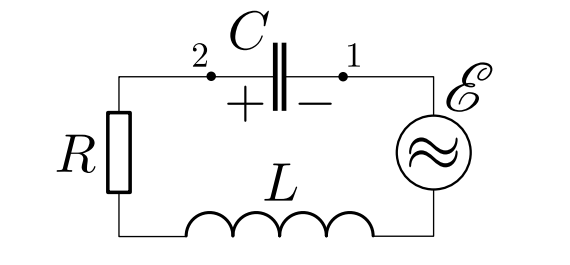
\includegraphics[width=0.8\textwidth]{./img/scheme.png}
	\caption{Схема установки}
\end{figure}
